\section{Experiments}
\label{sec:experiments}

All experiments are reproducible from the released code with fixed
seeds. Real data: the ENIGMA-toolbox release of the Human Connectome
Project group-average cortical functional connectome, Schaefer-200
parcellation \citep{lariviere2021enigma,schaefer2018local,vanessen2013wu},
five years of daily closes for S\&P~500 constituents (2013--2018), and
a U.S.\ air-traffic flow network. A download script for the
subject-level ABIDE cohort \citep{craddock2013neuro,dimartino2014autism}
accompanies the code; the cohort analysis of
Section~\ref{sec:exp-cohort} is synthetic, calibrated to connectomic
dimensions and labeled as such. Supplement Section~S4 details sources,
preprocessing, and testing conventions.

\subsection{Emergence of spikes and the finite-$n$ boundary}
\label{sec:exp-bbp}

Supplement Figure~S1 verifies the eigenvalue prediction of
Proposition~S2 at $n=2000$; Figure~\ref{fig:bbp} shows the
fixed-array reading, which is the reading the paper uses. Eight realizations of the ergodic array with
$\blam=(0.28,0.14,0.07)$, $\sigma=1$ were generated once at $n=1600$,
and the eigenvalues of their nested corners were computed as $n$
grows: each curve tracks one fixed network observed on more nodes. The effective spikes $s_k=\sqrt n\,\lam_k$ cross the transition in
turn: the third eigenvalue is indistinguishable from the bulk at
$n=100$ (mean $1.87$ against a bulk edge estimate of $1.86$) and is
resolved by $n=800$ ($2.40$ against the prediction $2.48$; $3.14$
against $3.16$ at $n=1600$). The corner resolves additional eigenvalues as $n$ grows.

\begin{figure}[t]
\centering
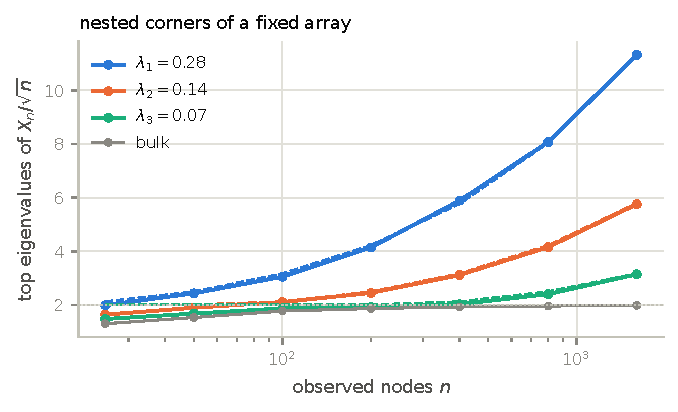
\includegraphics[width=0.54\textwidth]{figures/fig1_bbp.pdf}
\caption{Finite-$n$ calibration: top four eigenvalues of
$X_n/\sqrt n$ for nested corners of fixed arrays
($\blam=(0.28,0.14,0.07)$, $\sigma=1$; mean over 8 arrays generated
once at $n=1600$); dashed curves are $s_k+1/s_k$; the gray series is
the bulk edge. Supplement Figure~S1 shows the matching check of the
eigenvalue prediction at $n=2000$.}
\label{fig:bbp}
\end{figure}


\subsection{Level and power of the exact test}
\label{sec:exp-test}

Figure~\ref{fig:test}(a) measures the size of the hollow pipeline,
which Remark~\ref{rem:hollow} identifies as approximate: every matrix,
observed and replicate, is diagonal-zeroed before statistics are
computed. Across 250 null draws from spiked ensembles (spike count uniform on
$\{0,1,2,3\}$, magnitudes i.i.d.\ $U(1.2,3)$, Haar directions;
$n=120$, $B=99$; full specification in the released code), the conditional $p$-values of all
five statistics are uniform, and the Bonferroni-combined test rejects
at rate $0.068$ at nominal $0.05$ ($17/250$; Wilson 95\% interval
$[0.043,0.106]$): the approximation gap is within Monte Carlo error of
zero at this $n$. Because every applied matrix in this paper is a
finite-$T$ sample correlation or a transformed flow network, we also
measured the correlation pipeline, where the unit diagonal constrains
the matrix to the elliptope. For $T\times n$
panels of i.i.d.\ $N(0,1)$ entries with $n=120$, Fisher-$z$ sample
correlations, and the full battery ($R=100$, $B=99$), the combined test rejected at rate $0.060$ for $T=120$ and $0.040$
for $T=360$, every per-statistic rate at most $0.06$ (Supplement
Table~S1): the distortion from the elliptope constraint is within
Monte Carlo error of zero, consistent with the perturbation heuristic
of Remark~\ref{rem:hollow}.

The same ensemble calibrates the null models a practitioner might use
instead. Holding the rotatable truth fixed, a weight-permutation null
($B=99$) rejects the combined battery in $0.51$ of replicates at
nominal $0.05$, the miscalibration carried by exactly the summaries
applied fields report, clustering $0.57$ and strength-CV $0.42$; a
parametric bootstrap from the fitted spiked model attains $0.03$
combined with per-statistic rates up to $0.10$, roughly calibrated at
the price of fitting the model class and with no finite-sample
guarantee (Supplement Table~S2). The conditional test fits nothing and
is calibrated for any observed spectral shape, market modes and
Marchenko--Pastur bulks included; fitted or rewired generative
ensembles \citep{maslov2002specificity} test a different null and are
exact for none, quantified by the $0.51$ rejection rate above.

Figure~\ref{fig:test}(b) shows power against three exchangeable,
non-rotatable alternatives: a spike whose eigenvector interpolates from
delocalized to localized on $\lceil n^{2/3}\rceil$ coordinates; a
rank-2 graphon-Gaussian model with smooth bounded eigenfunctions
$\cos(\pi u),\cos(2\pi u)$; and heteroskedastic noise with log-normal
node variances. Localization is detected by the IPR statistic (power
$0.82$ at $\eta=1$, $0.74$ at $\eta=0.75$) and variance structure by
strength-CV (power $1.0$ from $\eta=0.2$). The graphon curve stays near
size over the whole range (rejection rates $0.02$ to $0.08$), and even
tripling the graphon signal (spikes $5.0,2.5$ at $n=200$) yields
combined power of only $0.56$. The theory explains this power gap: such a graphon differs from a
rotatable law only through the non-Gaussian geometry of its
eigenfunctions, the observable eigenvector is diluted to overlap
$\sqrt{1-\sigma^2/\theta^2}$ (Proposition~S2(ii)), and below the transition no consistent test exists against the
spherical-prior analogue (Corollary~S2); the cosine-direction curve is
the empirical counterpart. This battery, at these sizes,
has little power against weak smooth delocalized graphons; the
detectable departures are localization and scale heterogeneity, the
channels that reject on the real networks below.

\begin{figure}[t]
\centering
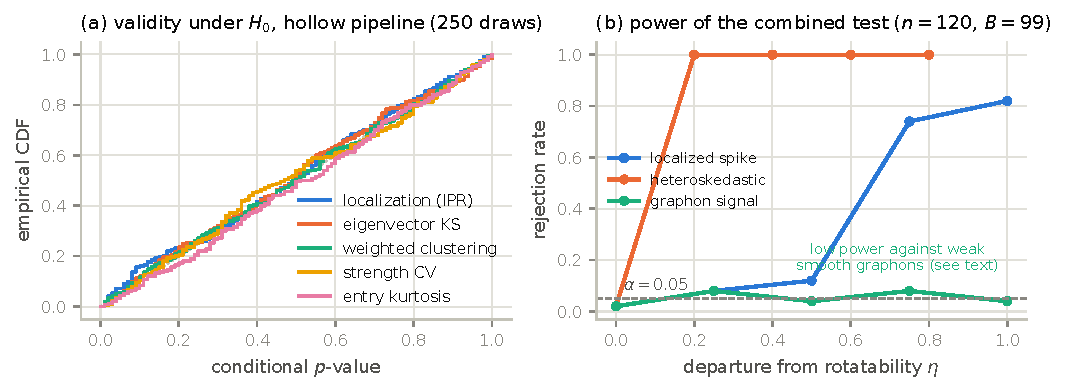
\includegraphics[width=0.92\textwidth]{figures/fig2_test.pdf}
\caption{The Haar-conditional rotation test. (a) Null $p$-value ECDFs
for the five statistics under the hollow pipeline (250 draws, $n=120$,
$B=99$); the diagonal is exact uniformity. (b) Power of the combined
battery against localized-spike, heteroskedastic, and smooth
graphon-Gaussian alternatives; the graphon alternative remains near
size (see text).}
\label{fig:test}
\end{figure}

\subsection{Real networks: which statistics reject, and what survives $G$}
\label{sec:exp-real}

\begin{table}[t]
\centering\small
\caption{Haar-conditional $p$-values (upper tail) on real networks,
before and after normal-scores Gaussianization $G$. HCP: group-average
functional connectome, Fisher-$z$, $n=200$, $B=499$. Air traffic:
$\log(1+\text{flow})$, $n=183$, $B=199$; the $G$ rows report ranges over
five tie-breaking seeds. S\&P~500: share of 28 rolling windows
(Fisher-$z$ correlations, $n=300$, $B=99$) with $p\le0.05$; modularity $p$-values were not computed per window (n/a here);
per-window modularity values enter the reconstruction study of
Section~\ref{sec:exp-cohort}. $p$-values near 1 indicate lower-tail
values (see text).}
\label{tab:real}
\begin{tabular}{llccccc}
\toprule
Network & version & IPR & clustering & modularity & strength CV & kurtosis\\
\midrule
HCP functional & raw & 0.004 & 0.836 & 1.000 & 1.000 & 0.002\\
 & after $G$ & 0.190 & 0.002 & 0.992 & 1.000 & 1.000\\
Air traffic & raw ($\log$) & 0.005 & 0.005 & 1.000 & 0.005 & 0.045\\
 & after $G$ & 0.005--0.020 & 0.005--0.010 & 1.000 & 0.005 & 1.000\\
S\&P 500 (share $p\le.05$) & raw & 0.25 & 0.75 & n/a & 0.00 & 0.25\\
 & after $G$ & 0.89 & 1.00 & n/a & 0.00 & 0.00\\
\bottomrule
\end{tabular}
\end{table}

Table~\ref{tab:real} and Figure~\ref{fig:real} report the test on
the three systems; all reject strict rotatability somewhere, as
expected, and the scientific content is in which statistics reject, in
the residuals, and in what survives $G$.

\emph{Human connectome.} The raw connectome rejects through localization
(IPR $p=0.004$, residual $z=+10.1$) and entry kurtosis ($p=0.002$,
$z=+89.7$), while the summaries network neuroscience most often reports
are not extreme in the upper tail: clustering sits inside its
conditional null ($p=0.836$, $z=-0.9$), and modularity and strength-CV
fall in the lower tail ($p\approx1$; $z=-16.6$ and $-10.3$). Given its
spectrum, the group-average connectome is less modular and less
strength-heterogeneous than a random rotation of that spectrum, and no
more clustered. After $G$ the localization rejection is no longer
significant ($p=0.190$) and kurtosis moves to the lower conditional tail
(upper-tail $p=1.000$), while a clustering
rejection appears ($p=0.002$): the marginal transform does not render every entry-level statistic consistent with the null. By the interpretation of Section~\ref{sec:diagnostic}, the localization
signal is consistent with a mainly tail-driven departure at this
resolution; group averaging can attenuate subject-level localization,
which the protocol of Section~\ref{sec:exp-cohort} measures on real
cohorts. This is one group-average matrix, a demonstration of the
method, with no claim about connectomes in general.

\emph{S\&P 500.} Across 28 rolling windows, strength-CV is uniformly
lower-tail (all windows at $p\ge0.95$) and kurtosis is lower-tail in
$0.68$: given spectra that include the market mode, the correlation
networks are more homogeneous in node strength than random rotations of
those spectra. Clustering rejects upper-tail in $0.75$ of raw windows
and all windows after $G$; IPR in $0.25$ raw and $0.89$ after $G$,
consistent with sector localization sharpened once the market-wide
scale is removed. These are per-window findings; windows overlap in
time.

\emph{Air traffic.} The log-flow network rejects through localization,
clustering, and strength-CV (all $p=0.005$), with kurtosis marginal
($p=0.045$) and modularity lower-tail. After $G$, repeated over five
tie-breaking seeds because most airport pairs have tied zero flows, kurtosis moves to the lower conditional tail (upper-tail $p=1.000$
at every seed) while
localization, clustering, and strength-CV persist at every seed (IPR
$p\in[0.005,0.020]$). The hub structure survives the marginal transform, consistent with
airline geography; the network is a positive control for the
diagnostic.

\begin{figure}[t]
\centering
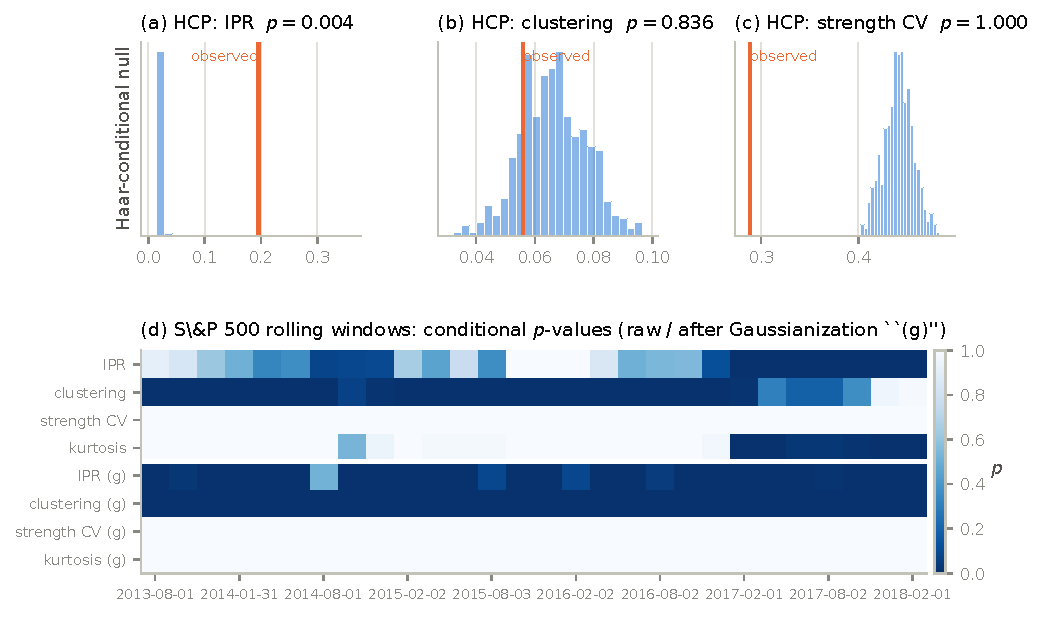
\includegraphics[width=0.92\textwidth]{figures/fig3_real.pdf}
\caption{Real networks. (a)--(c) HCP connectome: observed IPR,
clustering, and strength-CV against their Haar-conditional null
densities ($B=499$). (d) S\&P~500 rolling windows: conditional
$p$-values per window and statistic, raw and after Gaussianization.}
\label{fig:real}
\end{figure}

\subsection{Cohorts: sufficiency, residuals, and the protocol}
\label{sec:exp-cohort}

The cohort experiment implements the full protocol of
Sections~\ref{sec:sufficiency} and \ref{sec:test} on synthetic
cohorts calibrated to connectomic dimensions ($S=240$ subjects per
cohort, $n=200$, two groups). It validates the implementation of the
protocol and is evidence about the method, and about no real cohort;
the analysis environment could not reach the ABIDE bucket, and
Supplement Section~S4 specifies the identical pipeline, with fetch and
analysis code shipped, for the real data. Four feature sets enter
cross-validated logistic classifiers: spectral features, five
non-spectral summaries, the conditional residuals of those summaries
(Definition~\ref{def:residual}), and spectral plus summaries.

\emph{Cohort A: rotatable truth.} Both groups follow spiked
ensembles, the group difference planted in spike sizes. Spectral
features reach AUC $0.94\pm0.01$, raw summaries alone $0.89\pm0.01$
(marginally informative, as Remark~\ref{rem:scope} states), and adding
them to the spectrum gives no improvement ($0.93\pm0.01$). The
conditional residuals classify at chance ($0.46\pm0.02$): once each
subject's spectrum is conditioned out, the summaries carry no group
information. This is consistent with the parameter-free conditional
law of Corollary~S1; the marginal residual distribution can still vary
with the spectrum distribution, so chance-level classification is an
empirical finding here, and conditional-rank features give the exactly
invariant version. Per-subject
rotatability tests (Bonferroni at level $0.05$, 20 subjects per group)
reject for $0.00$ and $0.10$ of subjects, consistent with the level.

\emph{Cohort B: non-rotatable truth.} The spike-size distributions are
identical in the two groups, and group 1's leading eigenvector is
localized on 20 nodes. Spectral features classify at chance ($0.51\pm0.02$) while the
summaries and their residuals both reach AUC $1.00$: what the
summaries add is exactly a rotatability violation, and the residuals
isolate it. The per-subject test rejects
for $0.10$ of group-0 subjects and $1.00$ of group-1 subjects, so the
protocol of testing first and classifying on residuals second
identifies both the violation and the subjects carrying it.

\emph{S\&P 500 reconstruction.} Figure~\ref{fig:suff}(c) reports the
leave-one-out $R^2$ of predicting each summary of each rolling window
from six eigenvalue features of the same window: clustering $0.99$,
modularity $0.93$, kurtosis $0.82$, strength-CV $0.25$, IPR $0.03$. Two caveats: the windows overlap, so these are descriptive
within-sample associations, and the near-perfect reconstruction of
clustering is partly mechanical, since with one dominant market mode
clustering tracks the mean correlation level and hence $\lam_1$; the
result quantifies how much of each summary the spectrum determines,
the point of Corollary~S1, with no causal or predictive content.
The two summaries the eigenvalues fail to reconstruct, IPR and
strength-CV, are exactly the localization and scale statistics that
carry the conditional rejections in Table~\ref{tab:real}.

\begin{figure}[t]
\centering
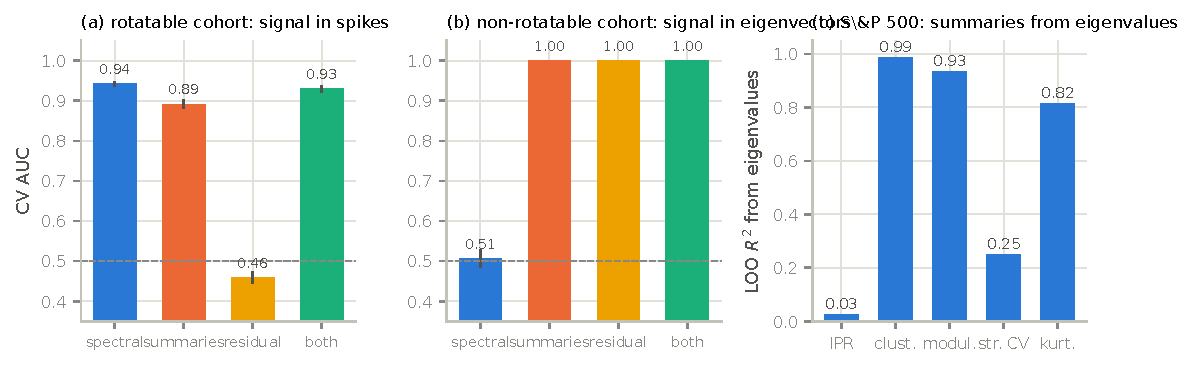
\includegraphics[width=0.92\textwidth]{figures/fig4_suff.pdf}
\caption{Cohorts and reconstruction. (a) Rotatable cohort: CV AUC on
spectral features, raw summaries, conditional residuals, and spectral
plus summaries; residuals are at chance. (b) Non-rotatable cohort
(localized eigenvector in group 1): spectral features are at chance;
summaries and residuals classify perfectly. (c) Leave-one-out $R^2$ of
predicting each summary of each S\&P~500 window from eigenvalue
features of the same window (descriptive; windows overlap).}
\label{fig:suff}
\end{figure}

\subsection{Nodewise attribution with exact familywise control}
\label{sec:exp-nodewise}

The nodewise protocol of Section~\ref{sec:test} was run on both real
networks, matching the Table~\ref{tab:real} pipelines
(Fisher-$z$ connectome, log-flow air network), with $\ell_i$ the
energy of node $i$ in the $K=10$ leading eigenvectors and $B=499$. On
the connectome, $8$ of $200$ parcels are flagged at familywise level
$0.05$ (global $p=0.008$), concentrated in two contiguous index
blocks of the Schaefer-200 ordering (parcels $12$--$13$ and
$102$--$113$): the aggregate IPR rejection of Table~\ref{tab:real}
is attributed to a short list of named parcels with an exact error
guarantee. On the air-traffic network, $8$ of $183$ airports are
flagged (global $p=0.006$): DEN, IAH, DFW, ORD, ATL, MSP, DTW, and
SLC, the major national hubs, so the attribution recovers the known
hub geography. In both cases the protocol turns an aggregate
localization rejection into a familywise-controlled list of nodes,
the output Section~\ref{sec:intro} argues applied work should
report.

\subsection{Heavy tails and the diagnostic}
\label{sec:exp-heavy}

Supplement Figure~S1(a) compares edge-weight tails: a spiked GOE draw
(Hill index $6.1$; fixed top-$5\%$ threshold, sensitivity analysis
deferred), the spiked $1.5$-stable law of
Theorem~\ref{thm:stable} (Hill $1.2$), and the raw air-traffic flows
(Hill $2.9$); the delocalized-spike stable control below has Hill
$1.6$. Supplement Figure~S1(b) applies the diagnostic of
Section~\ref{sec:diagnostic} to four networks; the synthetic ensembles
are tested as full matrices because their models specify diagonals, and
the hollow pipeline is used for the hollow air-traffic data (Supplement
Section~S3).

The Gaussian control rejects nothing before or after $G$. The
delocalized-spike stable control rejects kurtosis and IPR raw
($p=0.005$ each) and neither after $G$ (kurtosis $0.825$, IPR
$0.805$): a purely tail-driven violation, removed by the transform.
The Theorem~\ref{thm:stable} model rejects both raw ($p=0.005$);
after $G$ kurtosis moves to the lower conditional tail
(upper-tail $p=1.000$) while localization persists
($p=0.005$): heavy-tailed factors are genuinely $\ell_4$-localized,
the diagnostic reports it correctly, and the $p$-rotatable class with
nonzero spikes populates the persistent row. The
air-traffic network behaves like the factor model: kurtosis reverts
($p=1.000$ at all tie seeds) while localization persists
($p\le0.020$ at all seeds). The readout separates marginal,
transform-removable heaviness from persistent eigenvector structure; on
these data, air-traffic hubs are of the second kind.
